% Figure 1.3a: Giao thoa kế vuông pha sóng dò (Bản tiếng Việt)
\begin{tikzpicture}[
  >=Stealth,
  font=\small,
  blk/.style={draw=black!75, rounded corners=3pt, fill=blue!8, semithick, align=center, inner sep=3pt},
  mathnode/.style={draw=black!75, circle, fill=yellow!20, thick, inner sep=1pt, minimum size=6.5mm},
  accum/.style={draw=black!75, rounded corners=3pt, fill=teal!12, semithick, align=center, inner sep=3pt},
  outnode/.style={draw=black!85, rounded corners=3pt, fill=green!12, thick, align=center, inner sep=3pt},
  wavebox/.style={draw=black!60, fill=white, thin, inner sep=2pt, align=center},
  arrow/.style={->, thick, black!75}
]

% Khung đầu vào
\node[blk, fill=blue!10, text width=2.4cm] (input) at (1.3, 0) {
  \textbf{Khung đầu vào}\\
  $x_\ell[n]$\\
  \scriptsize $0 \le n < N$ ($N{=}512$)
};

% Điểm rẽ nhánh
\coordinate (split) at (3.0, 0);
\filldraw[black!80] (split) circle (2.2pt);
\draw[arrow] (input) -- (split);

% Tách hai nhánh trực giao
\coordinate (c_in) at (3.0, 0.9);
\coordinate (s_in) at (3.0, -0.9);
\draw[thick, black!75] (split) -- (c_in);
\draw[thick, black!75] (split) -- (s_in);

% Nhánh trên: Cosine (Đồng pha)
\node[mathnode] (mul_cos) at (4.9, 0.9) {\large $\times$};
\draw[arrow] (c_in) -- (mul_cos);

\node[wavebox, text width=2.7cm] (probe_cos) at (4.9, 1.85) {
  \scriptsize\textbf{Đồng pha} $\cos\left(\frac{2\pi k n}{N}\right)$\\[0.3mm]
  \begin{tikzpicture}[scale=0.18]
    \draw[->, gray!60] (0,0) -- (6.0,0);
    \draw[blue!75!black, thick, domain=0:6.28, samples=30] plot (\x, {sin(\x r + 1.57 r)});
  \end{tikzpicture}
};
\draw[arrow, blue!75!black] (probe_cos) -- (mul_cos);

\node[accum, text width=2.5cm] (acc_cos) at (8.1, 0.9) {
  \textbf{Bộ tích lũy}\\
  $\sum_{n=0}^{N-1} (\cdot)$\\[0.5mm]
  \scriptsize Tổng dồn
};
\draw[arrow] (mul_cos) -- (acc_cos);

\node[outnode, text width=2.4cm] (re_out) at (11.3, 0.9) {
  \textbf{Phần thực}\\
  $\text{Re}(X_\ell[k])$\\[0.5mm]
  \scriptsize Điểm đồng pha
};
\draw[arrow] (acc_cos) -- (re_out);

% Nhánh dưới: Sine (Vuông pha)
\node[mathnode] (mul_sin) at (4.9, -0.9) {\large $\times$};
\draw[arrow] (s_in) -- (mul_sin);

\node[wavebox, text width=2.7cm] (probe_sin) at (4.9, -1.85) {
  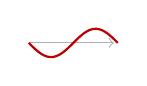
\begin{tikzpicture}[scale=0.18]
    \draw[->, gray!60] (0,0) -- (6.0,0);
    \draw[red!75!black, thick, domain=0:6.28, samples=30] plot (\x, {-sin(\x r)});
  \end{tikzpicture}\\[0.3mm]
  \scriptsize\textbf{Vuông pha} $-\sin\left(\frac{2\pi k n}{N}\right)$
};
\draw[arrow, red!75!black] (probe_sin) -- (mul_sin);

\node[accum, text width=2.5cm] (acc_sin) at (8.1, -0.9) {
  \textbf{Bộ tích lũy}\\
  $\sum_{n=0}^{N-1} (\cdot)$\\[0.5mm]
  \scriptsize Tổng dồn
};
\draw[arrow] (mul_sin) -- (acc_sin);

\node[outnode, text width=2.4cm] (im_out) at (11.3, -0.9) {
  \textbf{Phần ảo}\\
  $\text{Im}(X_\ell[k])$\\[0.5mm]
  \scriptsize Điểm vuông pha
};
\draw[arrow] (acc_sin) -- (im_out);

% Ghép thành bin phổ phức
\node[draw=purple!80!black, rounded corners=4pt, fill=purple!8, thick, align=center, text width=3.4cm] (euler) at (14.8, 0) {
  \textbf{Bin phổ phức}\\[0.8mm]
  $X_\ell[k] = \text{Re} + j\,\text{Im}$\\[1mm]
  \scriptsize \textbf{Vỏ bọc Euler:}\\[0.3mm]
  $\sum_{n=0}^{N-1} x_\ell[n]\, e^{-j\frac{2\pi kn}{N}}$
};

\draw[arrow, purple!80!black] (re_out.east) -- ++(0.3, 0) |- (euler.north west);
\draw[arrow, purple!80!black] (im_out.east) -- ++(0.3, 0) |- (euler.south west);

\end{tikzpicture}
